
\section{Code repository}
All our code can be found in the Jupyter notebook scripts \texttt{a.ipynb} and \texttt{b.ipynb} available in the folder \texttt{scripts} in the public repository at
\url{https://github.com/JackismyShephard/pml-22}.

\section{Extra figures}
\begin{figure}[!h]
	\begin{subfigure}[t]{1\textwidth}
		\centering
		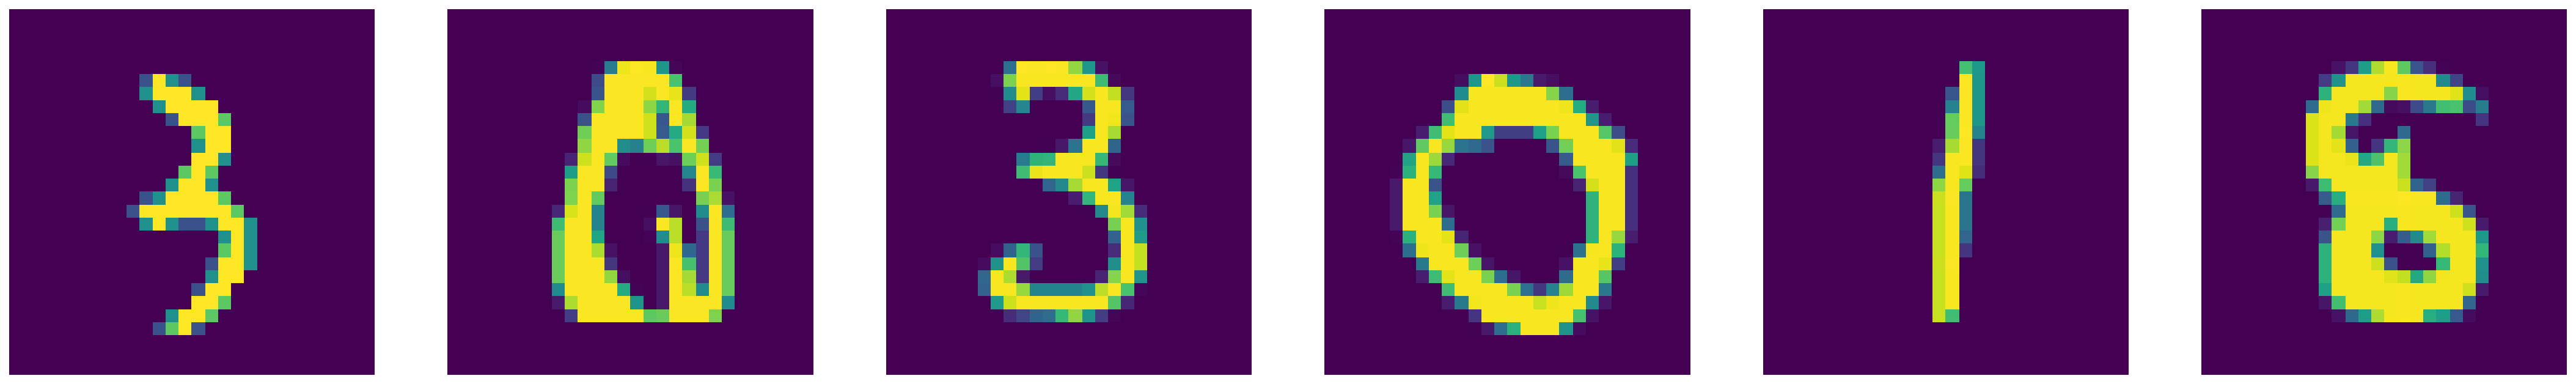
\includegraphics[width = 0.8\textwidth]{figures/ppca/real}
		\caption{Test set images}
	\end{subfigure}
	\begin{subfigure}[t]{1\textwidth}
		\centering
		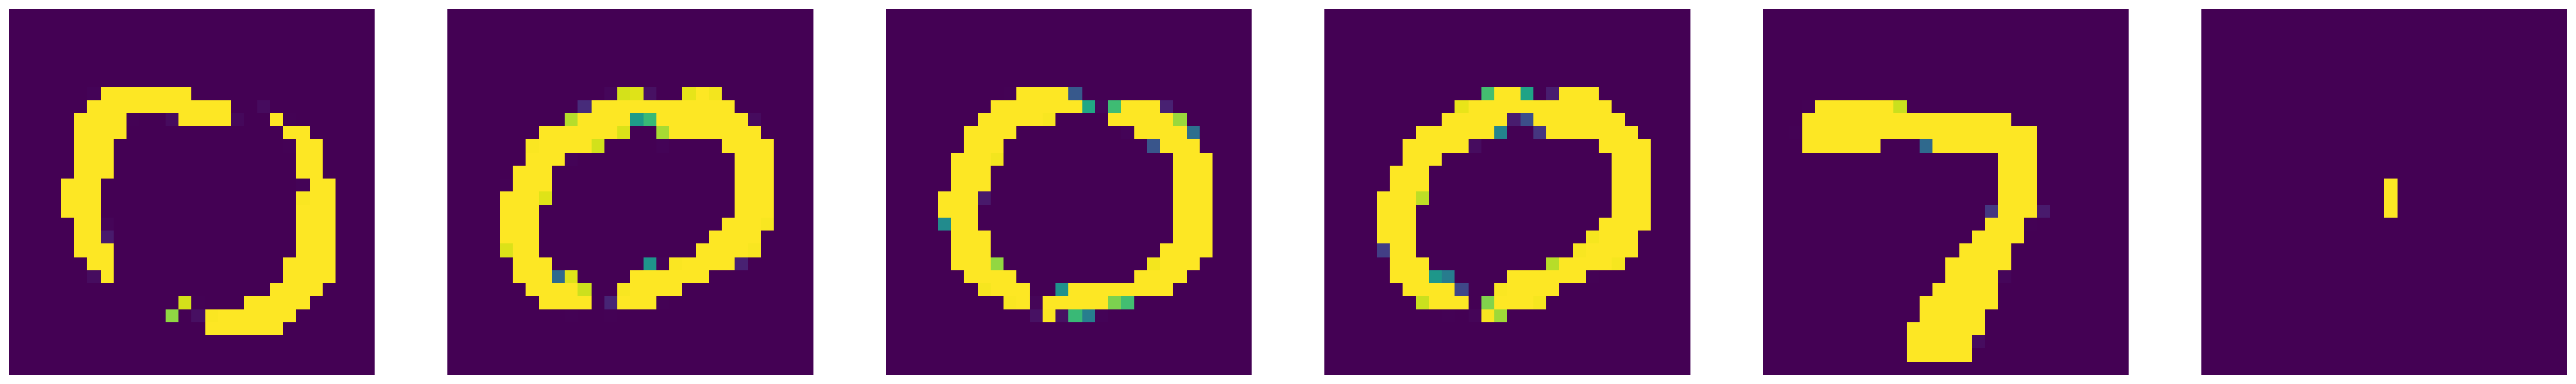
\includegraphics[width = 0.8\textwidth]{figures/vae/mean}
		\caption{VAE}
	\end{subfigure}
	\begin{subfigure}[t]{1\textwidth}
		\centering
		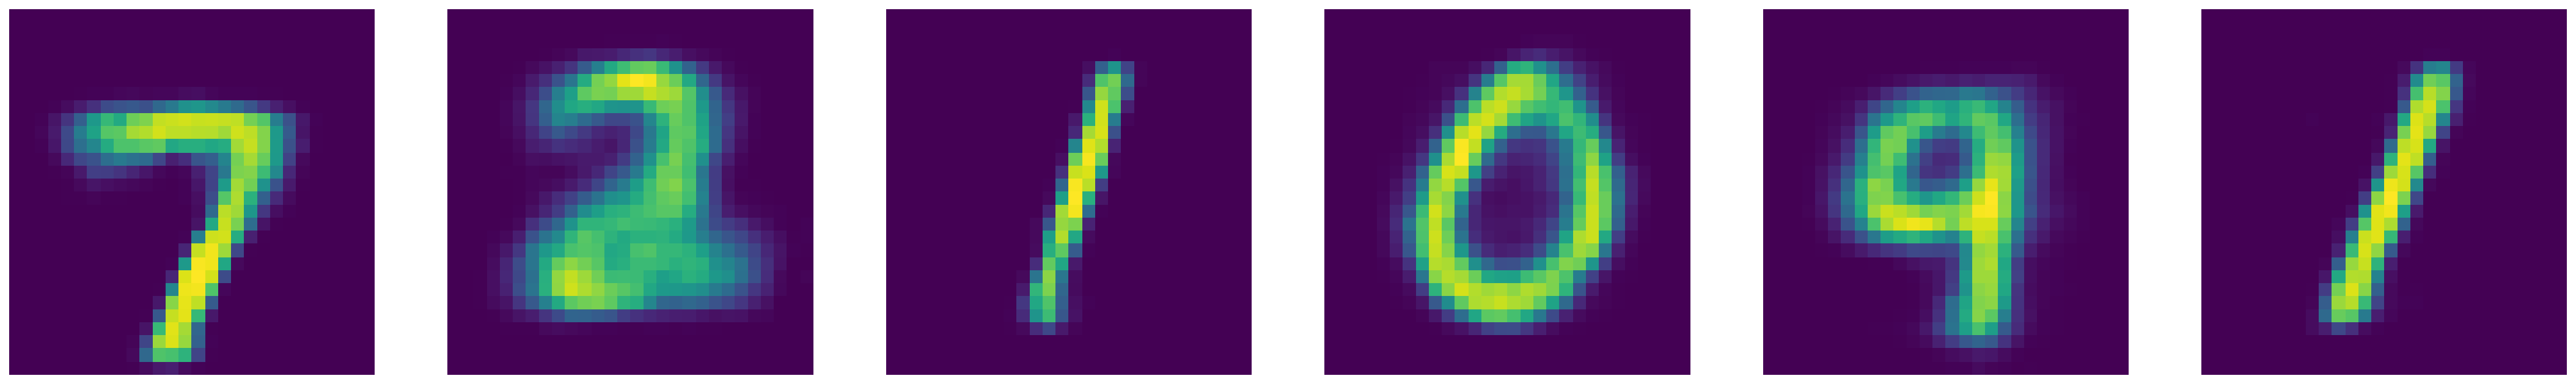
\includegraphics[width = 0.8\textwidth]{figures/cvae/mean}
		\caption{CVAE}
	\end{subfigure}
	\begin{subfigure}[t]{1\textwidth}
		\centering
		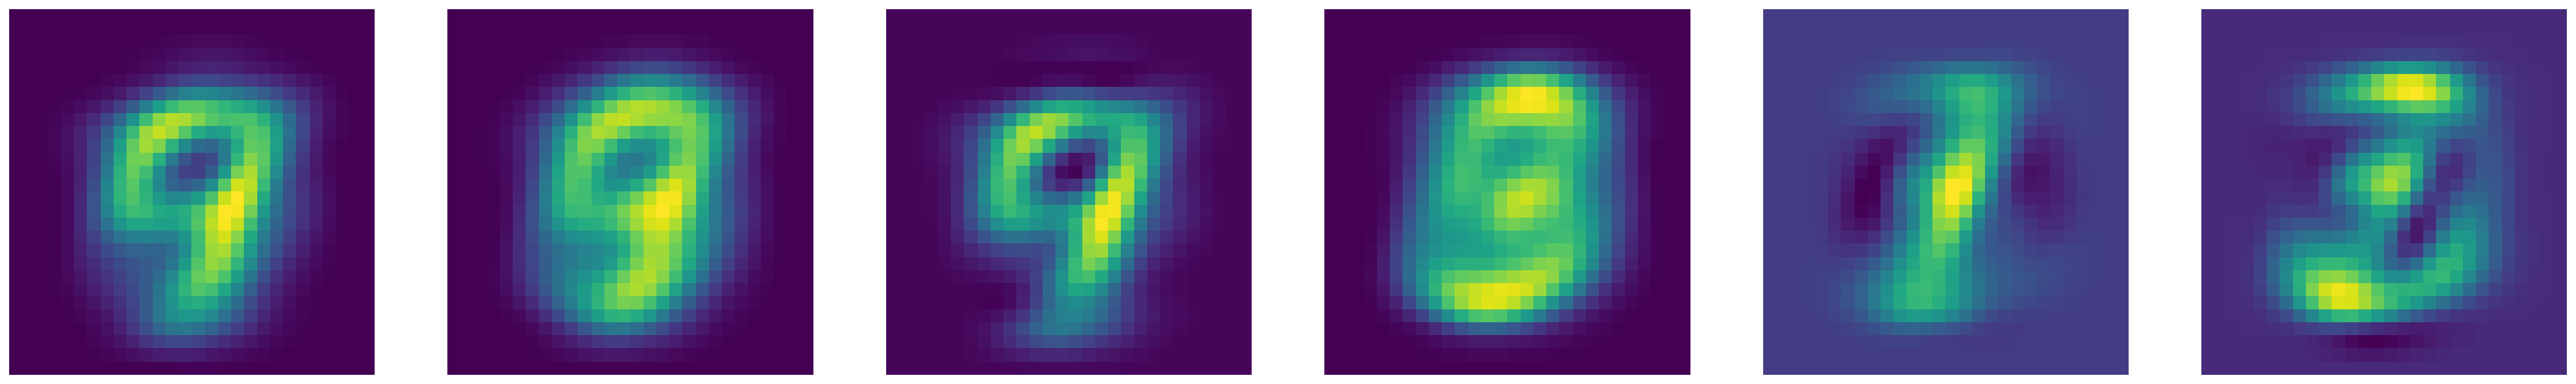
\includegraphics[width = 0.8\textwidth]{figures/ppca/mean}
		\caption{PPCA}
	\end{subfigure}
	\begin{subfigure}[t]{1\textwidth}
		\centering
		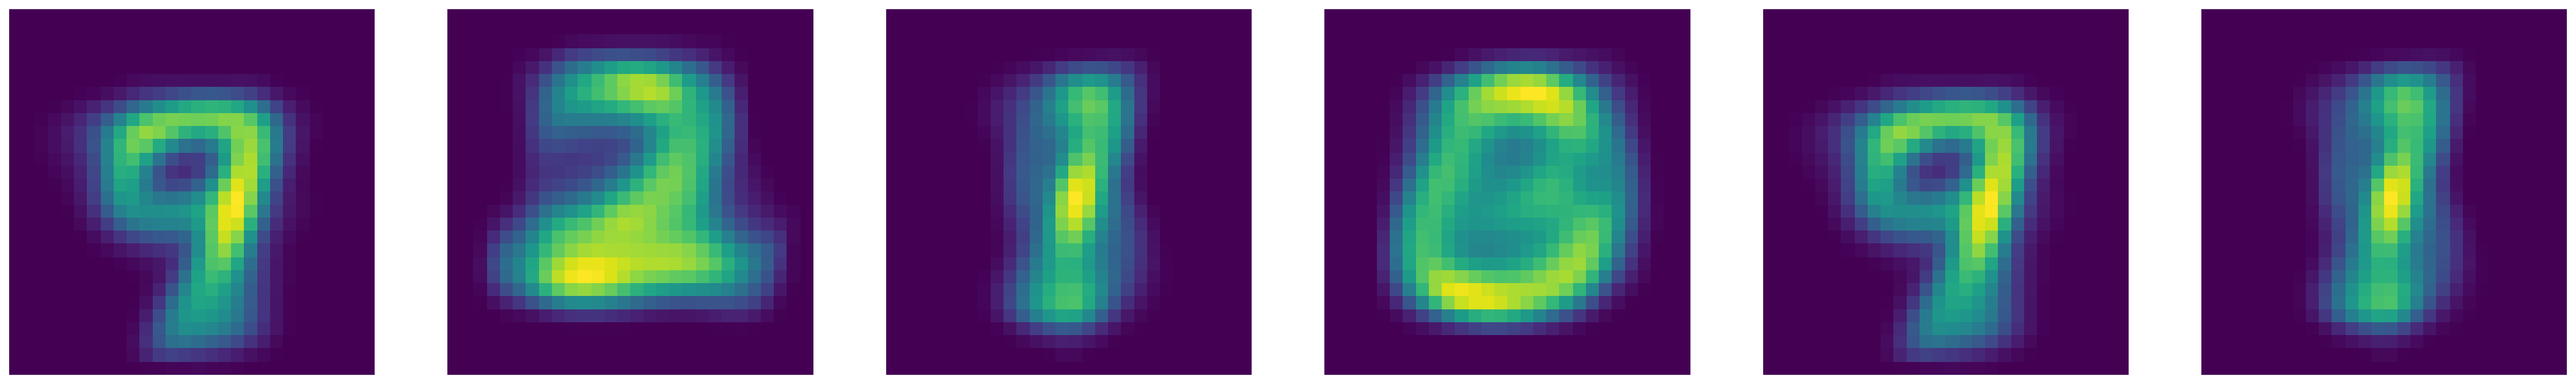
\includegraphics[width = 0.8\textwidth]{figures/gmm/mean}
		\caption{GMM}
	\end{subfigure}
	\caption{Comparison of MNIST test set images and corresponding reconstructions sampled from density models}
\end{figure}

\begin{figure}[!h]
	\begin{subfigure}[t]{0.49\textwidth}
		\centering
		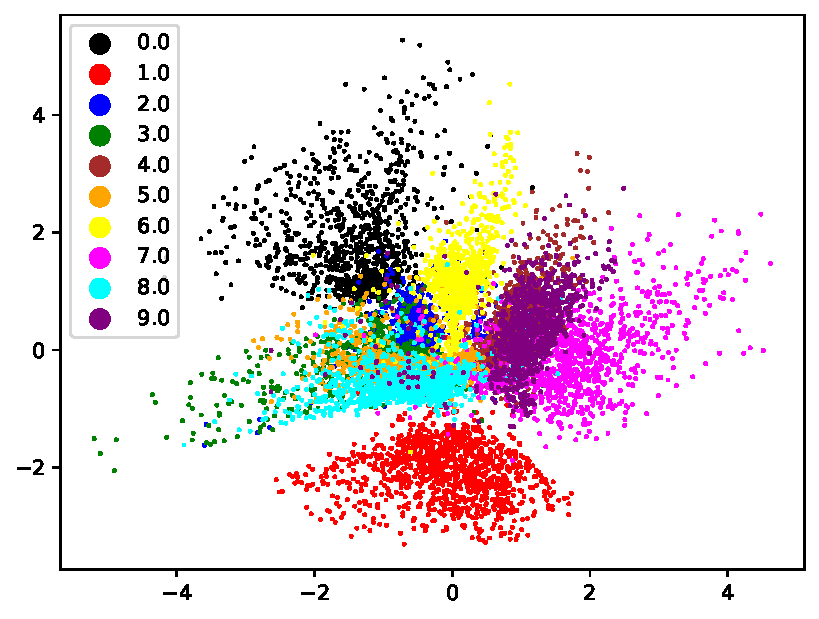
\includegraphics[width = 1\textwidth]{figures/vae/clustering}
		\caption{VAE}
	\end{subfigure}
	\begin{subfigure}[t]{0.49\textwidth}
		\centering
		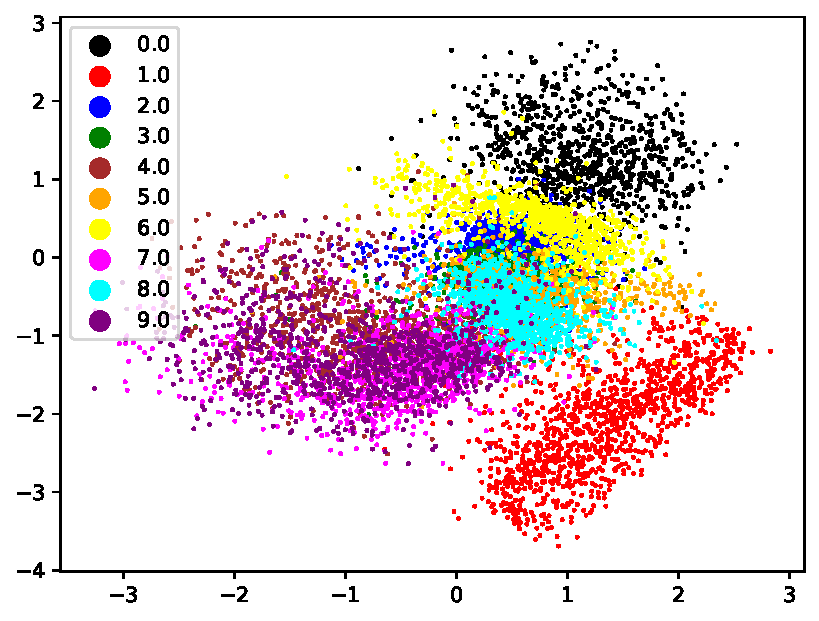
\includegraphics[width = 1\textwidth]{figures/cvae/clustering}
		\caption{CVAE}
	\end{subfigure}
	\begin{subfigure}[t]{0.49\textwidth}
		\centering
		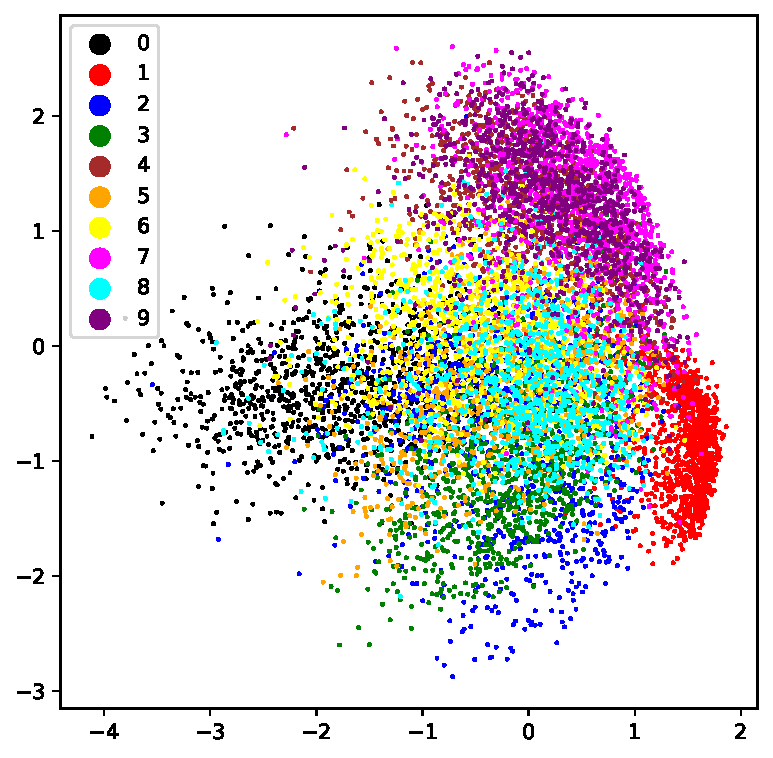
\includegraphics[width = 1\textwidth]{figures/ppca/clustering}
		\caption{PPCA}
	\end{subfigure}
	\begin{subfigure}[t]{0.49\textwidth}
		\centering
		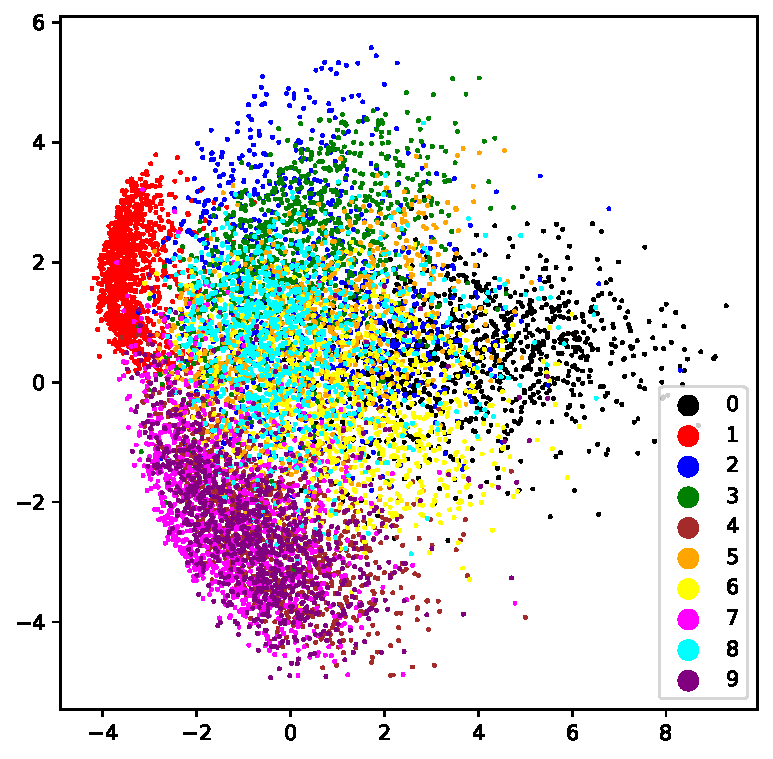
\includegraphics[width = 1\textwidth]{figures/gmm/clustering}
		\caption{GMM}
	\end{subfigure}
	\caption{Clustering on MNIST test (projection to latent space) using trained density models.}	
\end{figure}

\begin{figure}[!h]
	\begin{subfigure}[t]{0.49\textwidth}
		\centering
		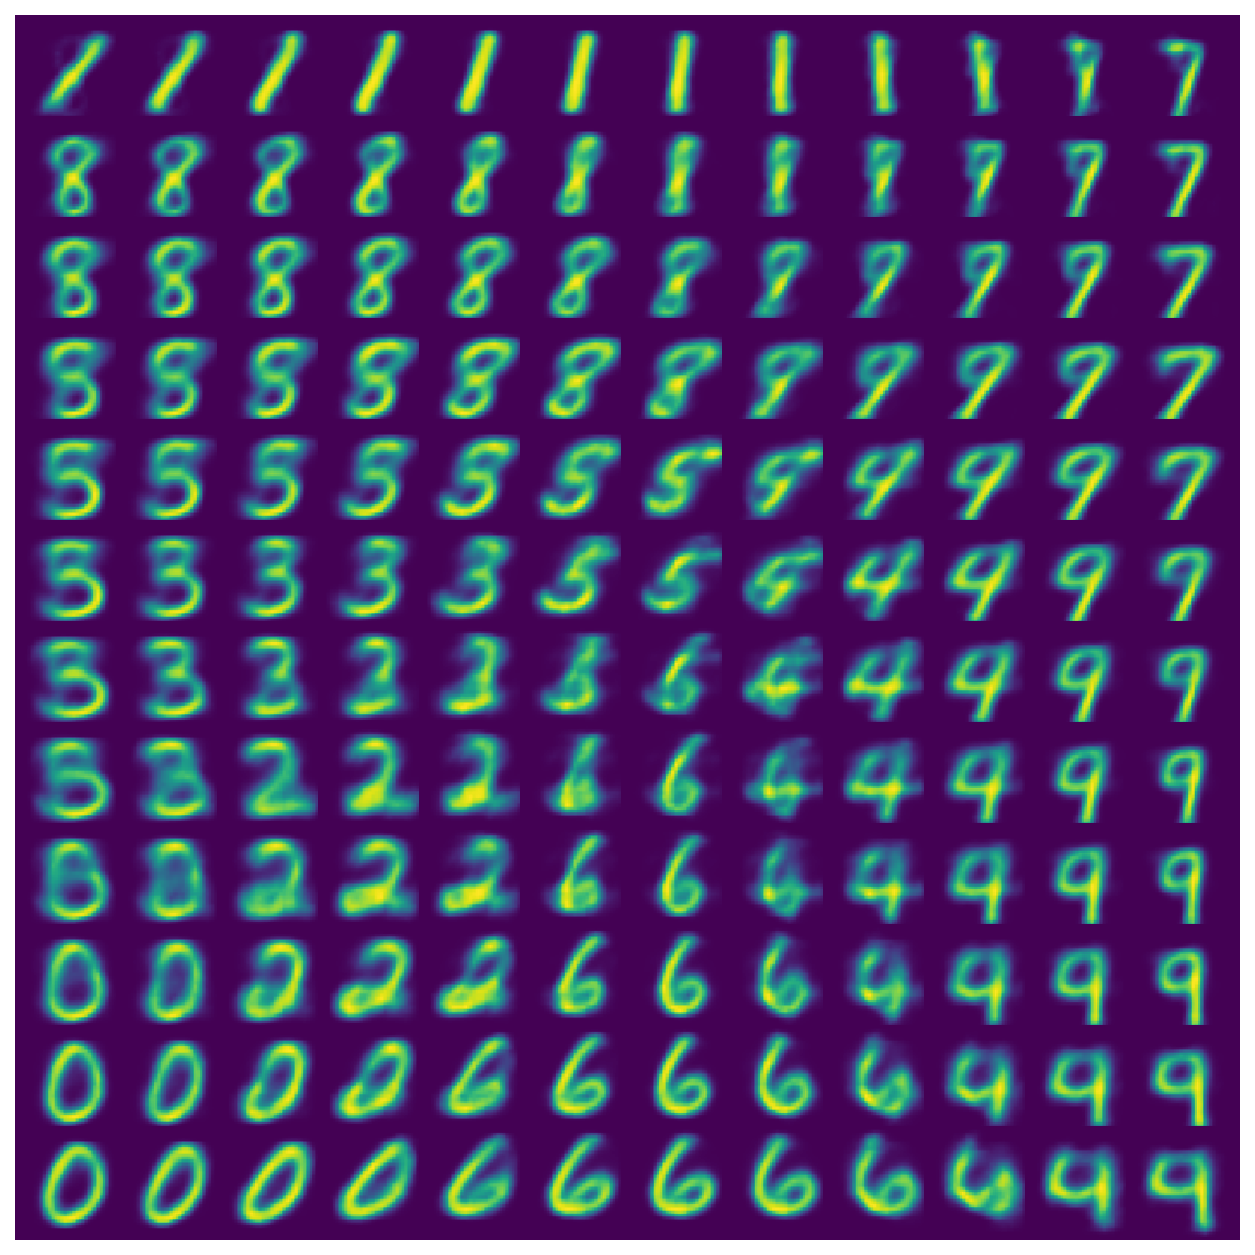
\includegraphics[width = 1\textwidth]{figures/vae/interpolation}
		\caption{VAE}
	\end{subfigure}
	\begin{subfigure}[t]{0.49\textwidth}
		\centering
		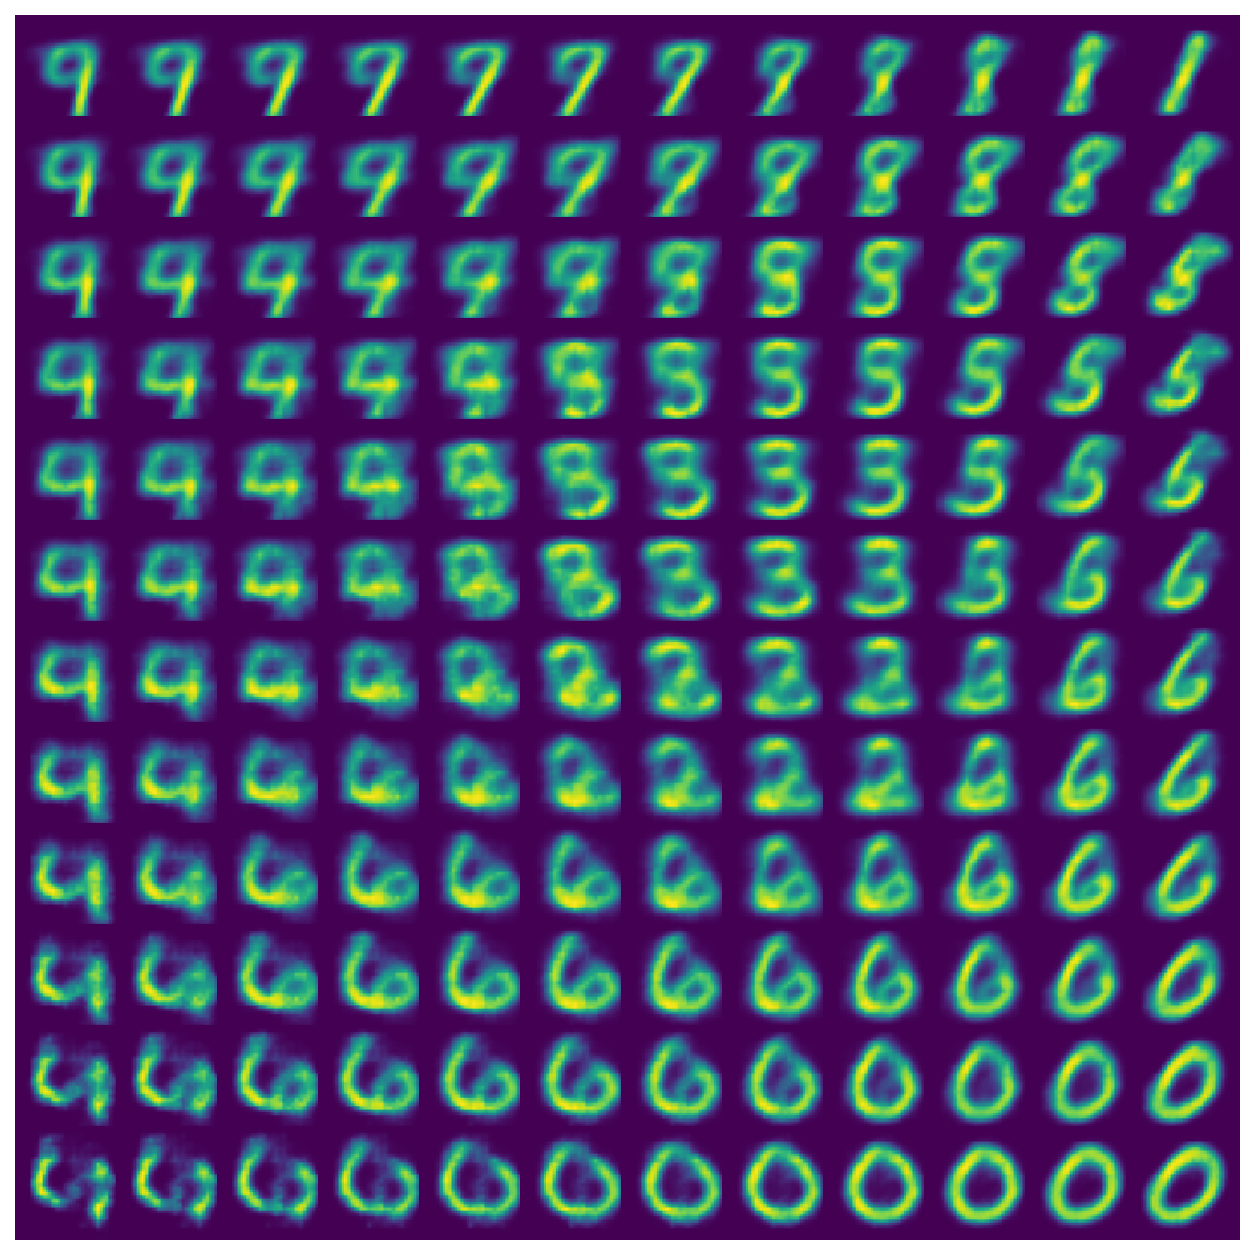
\includegraphics[width = 1\textwidth]{figures/cvae/interpolation}
		\caption{CVAE}
	\end{subfigure}
	\begin{subfigure}[t]{0.49\textwidth}
		\centering
		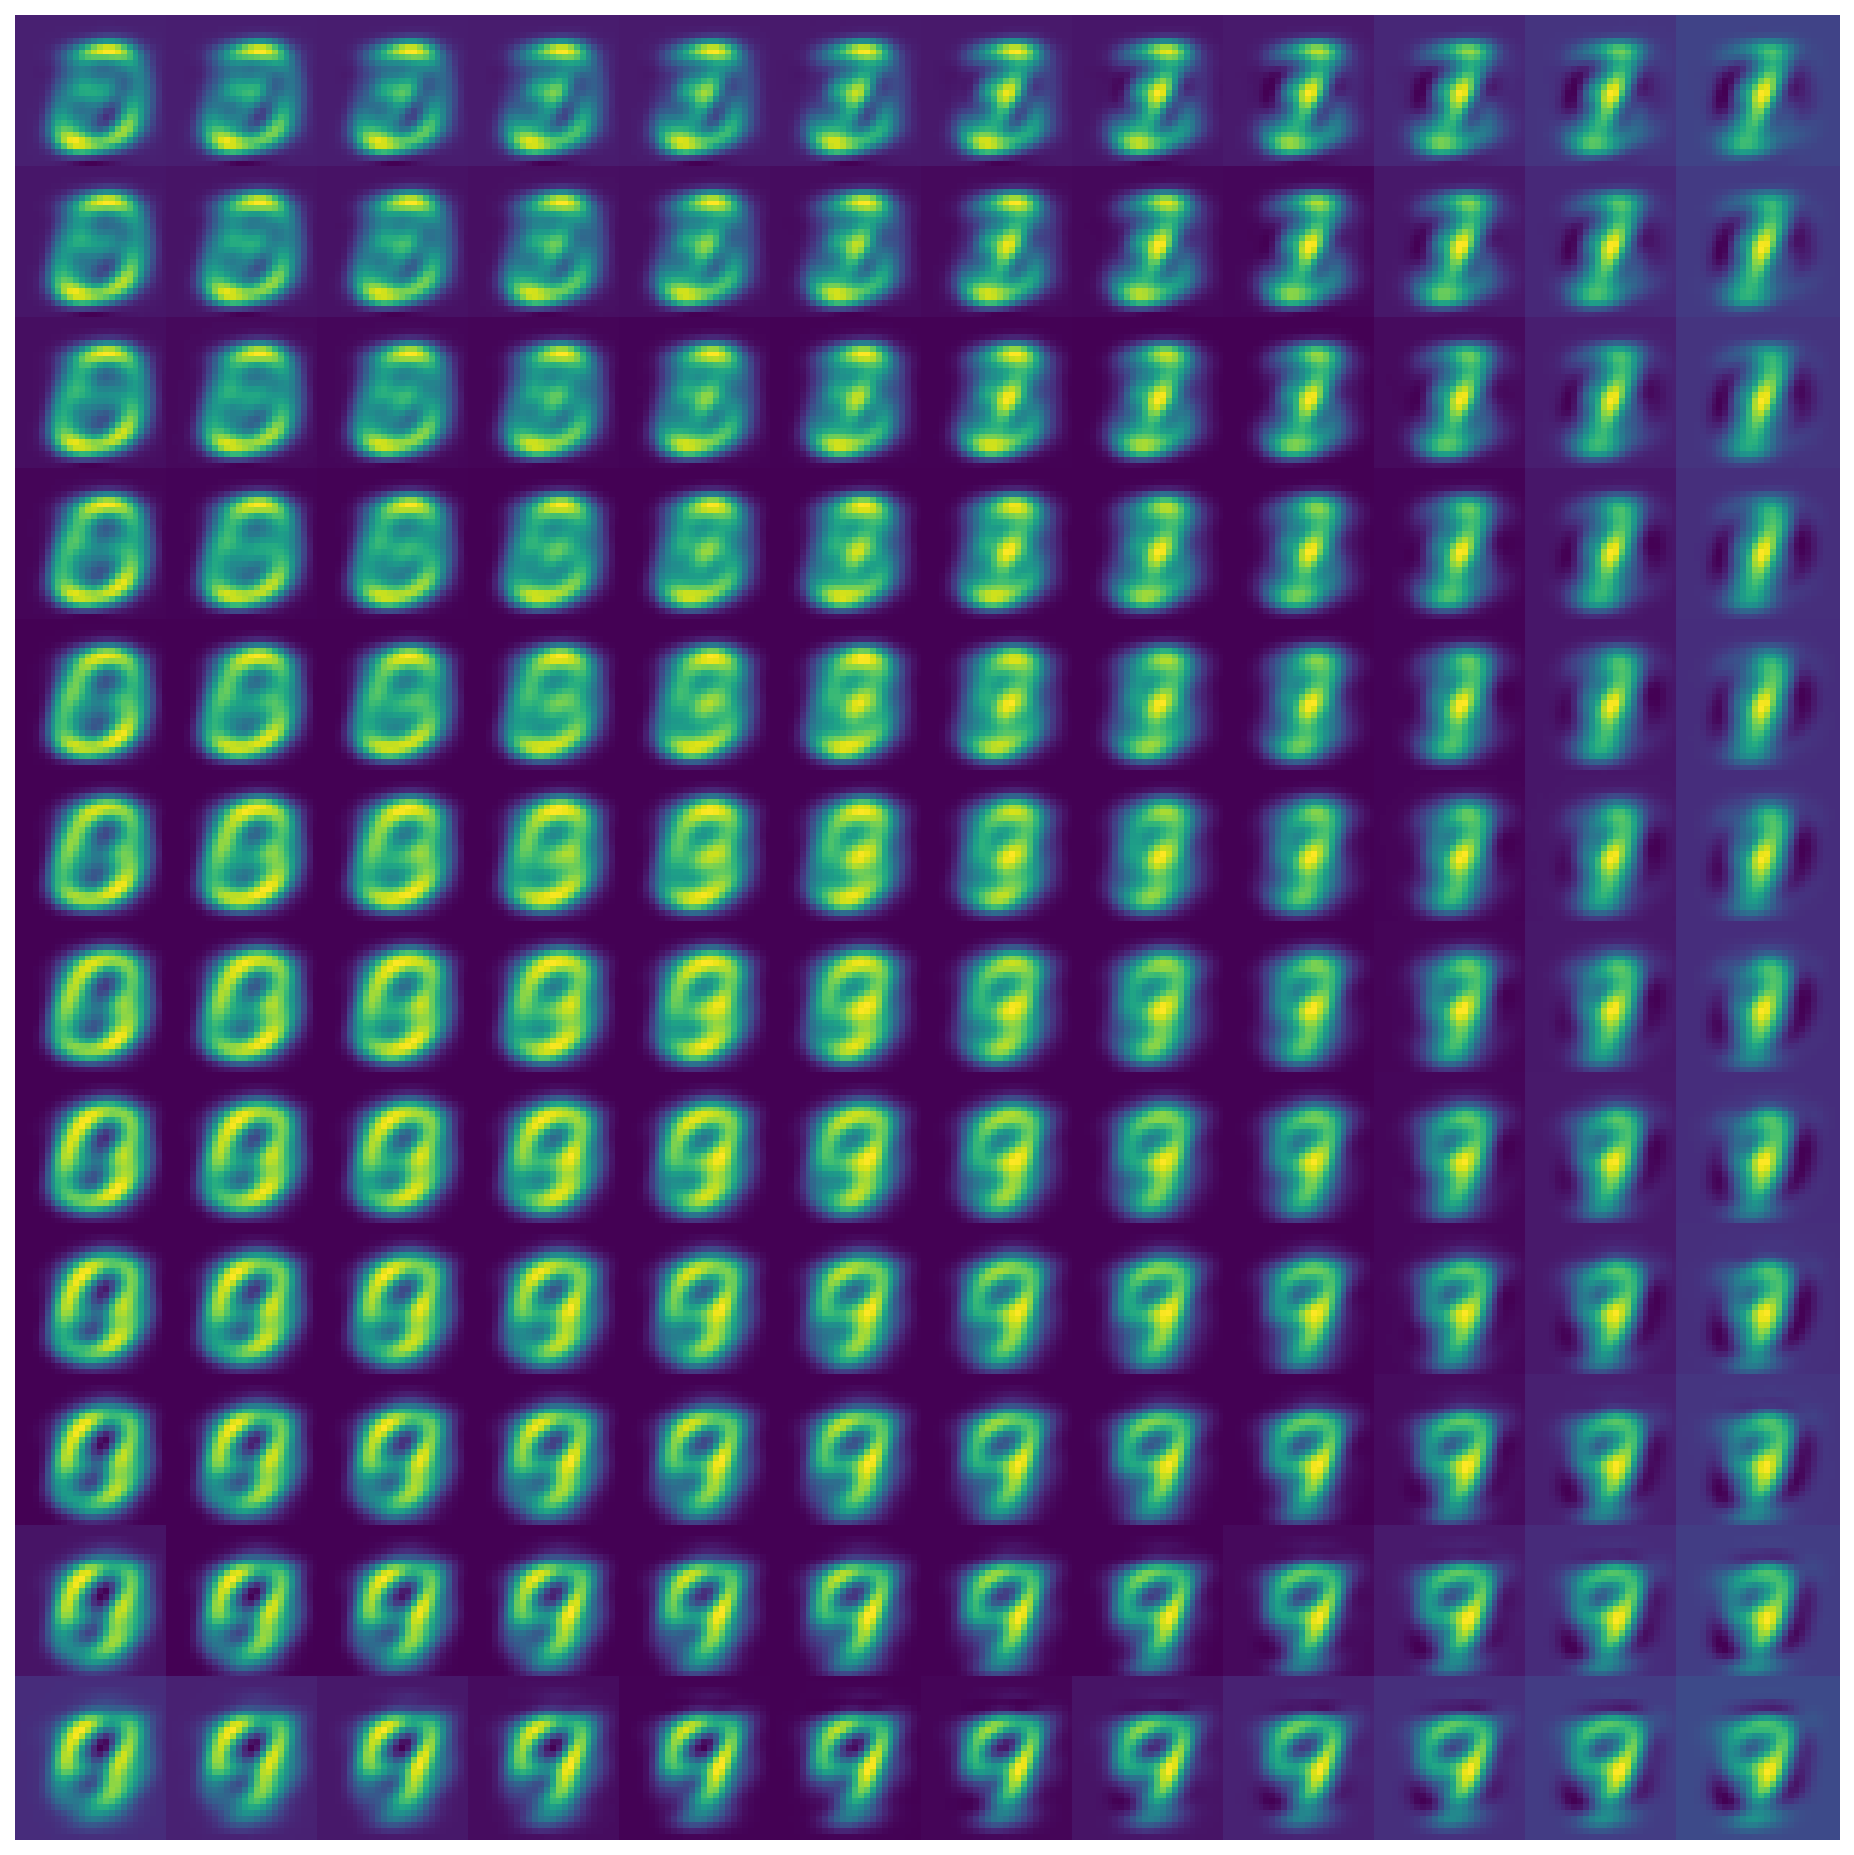
\includegraphics[width = 1\textwidth]{figures/ppca/interpolation}
		\caption{PPCA}
	\end{subfigure}
	\begin{subfigure}[t]{0.49\textwidth}
		\centering
		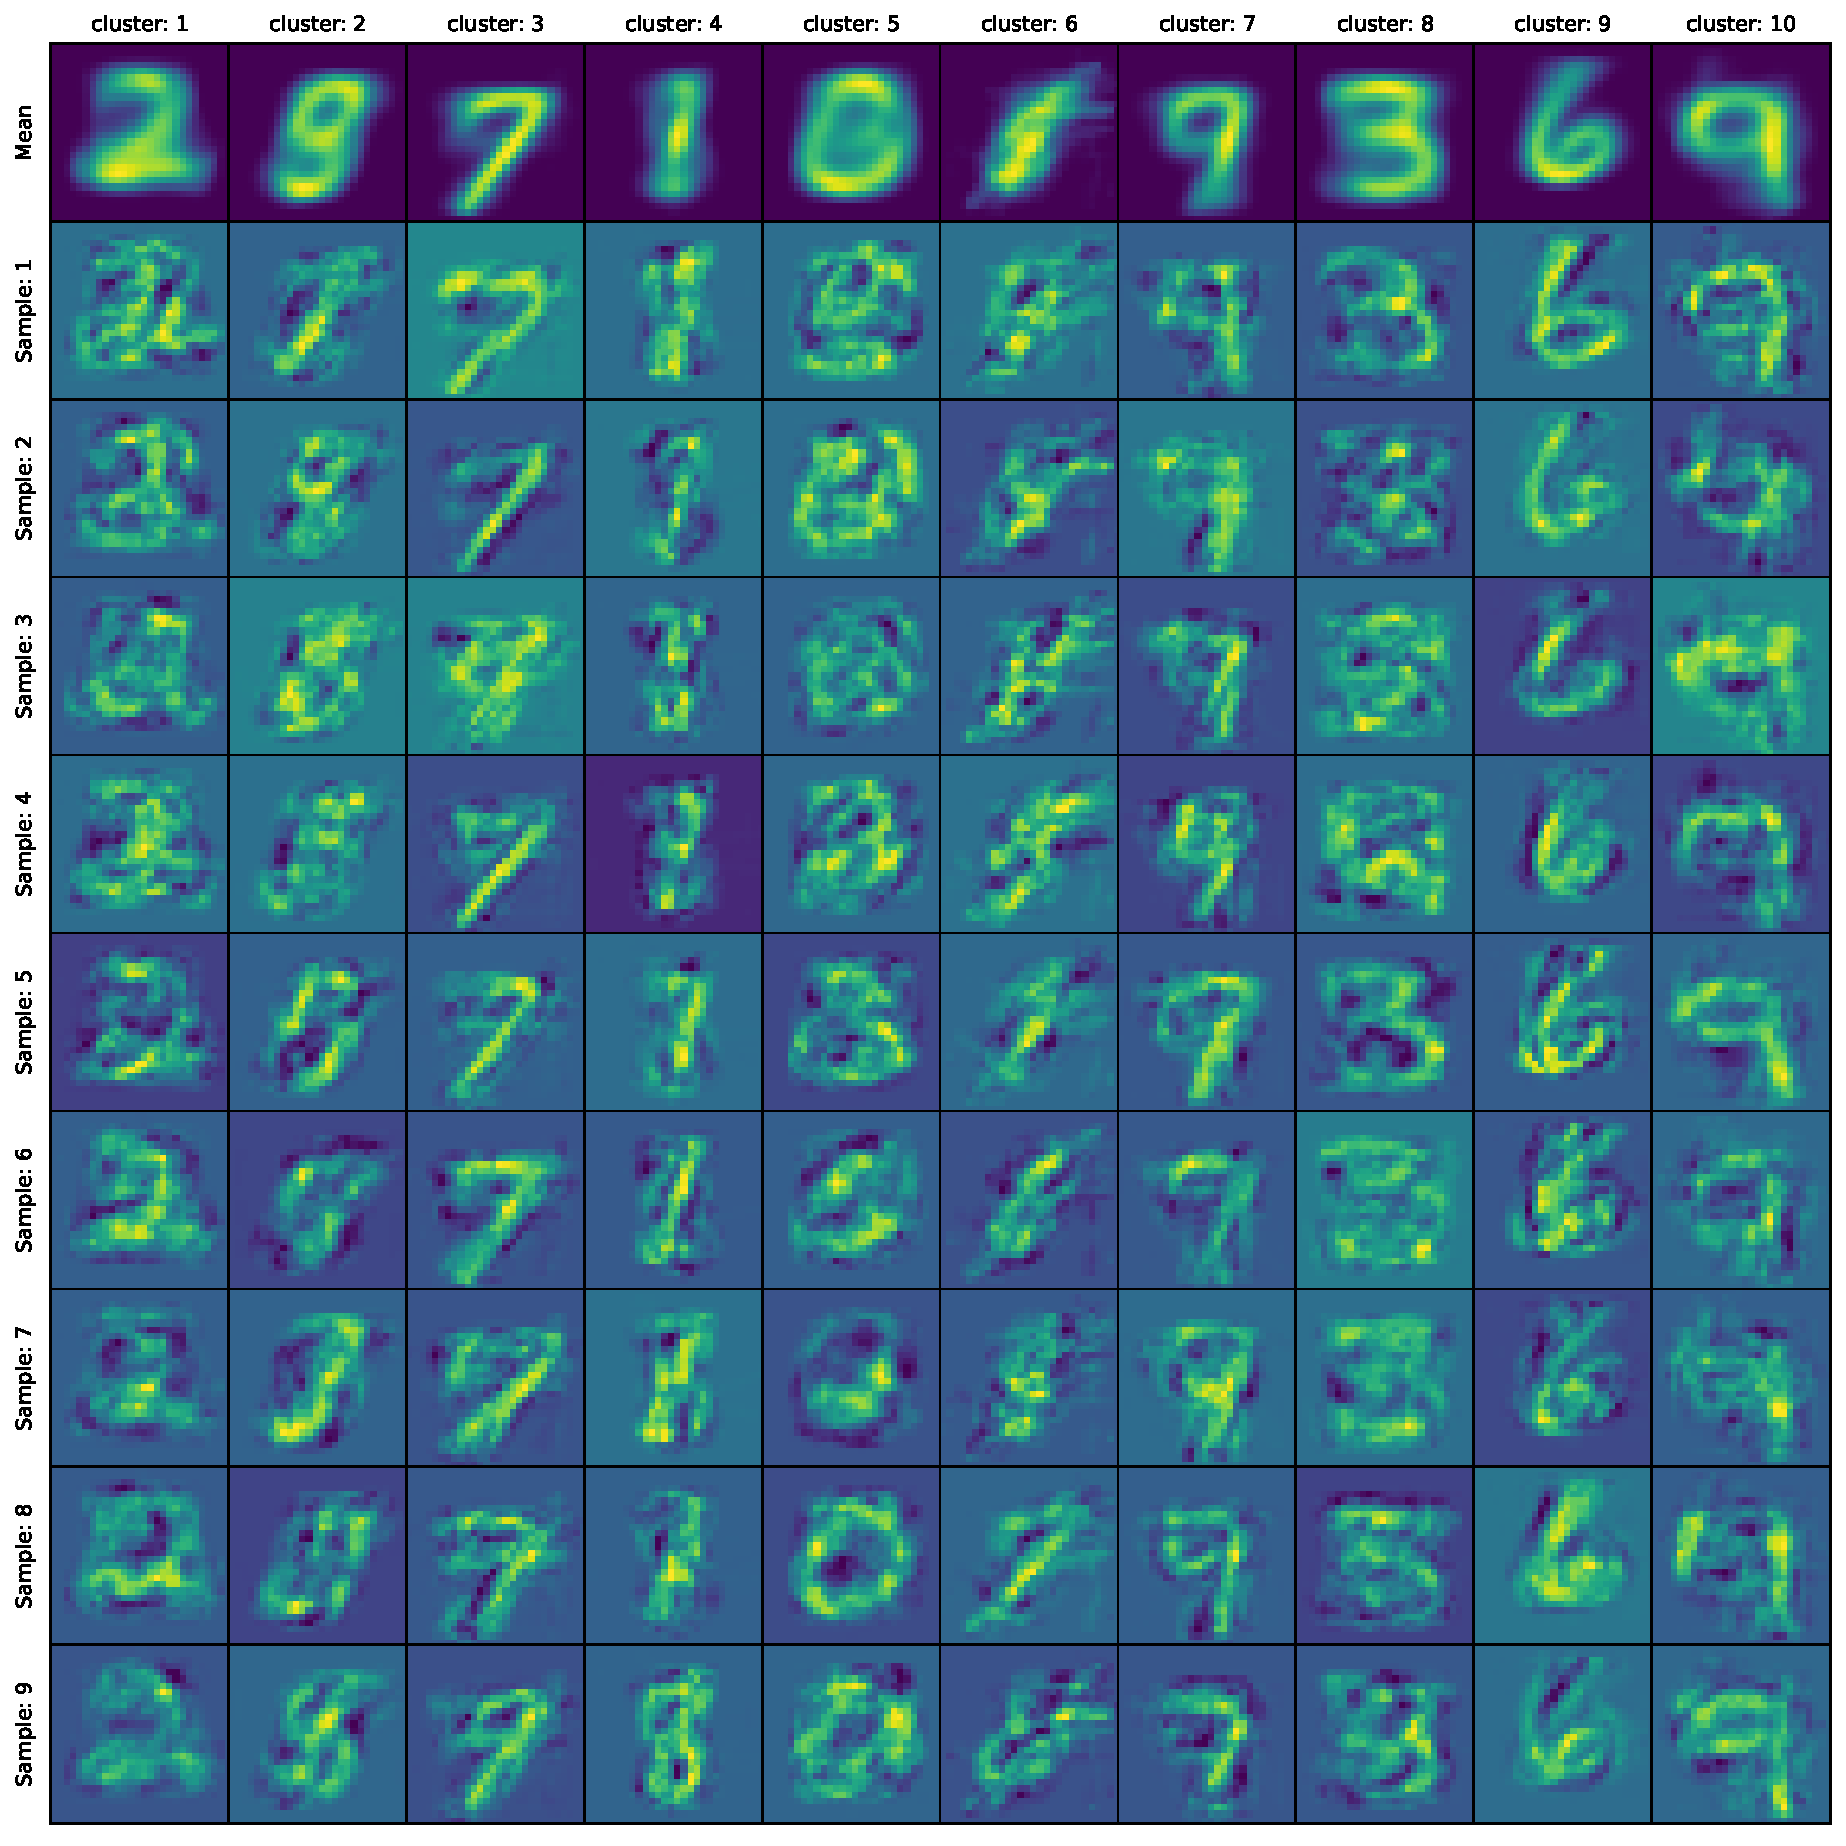
\includegraphics[width = 1\textwidth]{figures/gmm/interpolation}
		\caption{GMM}
	\end{subfigure}
	\caption{Interpolating images from latent space variables using trained density models}	
\end{figure}


\subsection{Bayesian optimization loop results}
\subsubsection{Large versions of plots from the B2 section of the report}
\begin{figure}[H]
    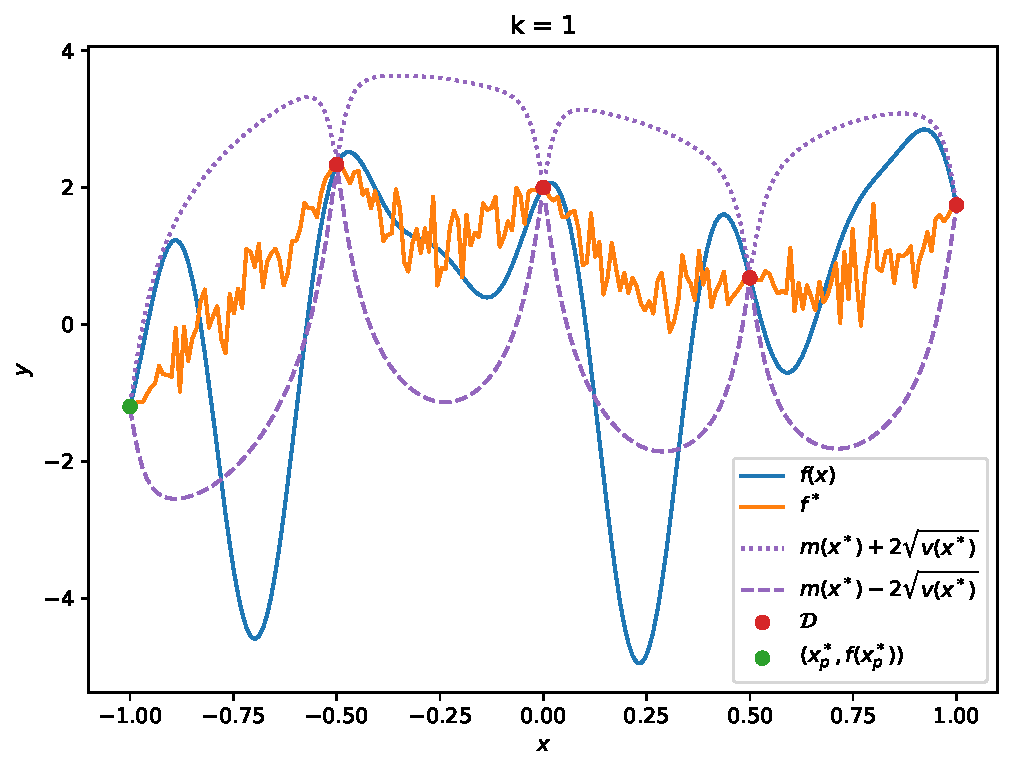
\includegraphics[width=\textwidth]{figures/gp/b2-k_1.pdf}
    \caption{Result of the Bayesian optimization loop with RBF kernel at iteration $k = 1$}
\end{figure}
\begin{figure}[H]
    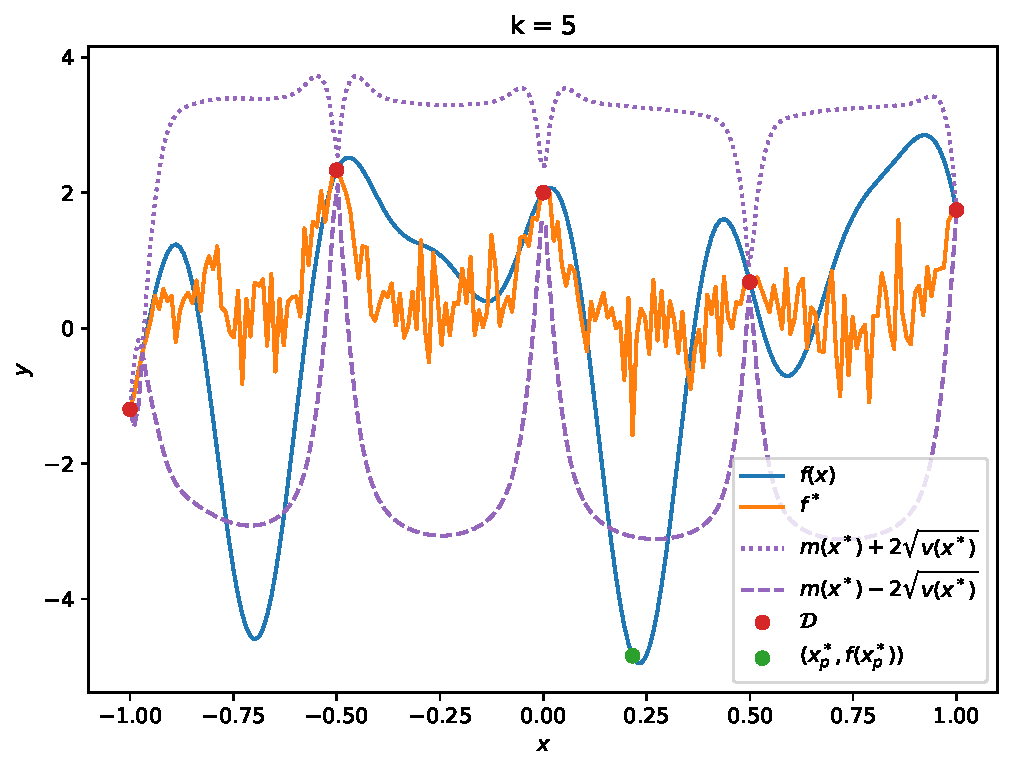
\includegraphics[width=\textwidth]{figures/gp/b2-k_5.pdf}
    \caption{Result of the Bayesian optimization loop with RBF kernel at iteration $k = 5$}
\end{figure}
\begin{figure}[H]
    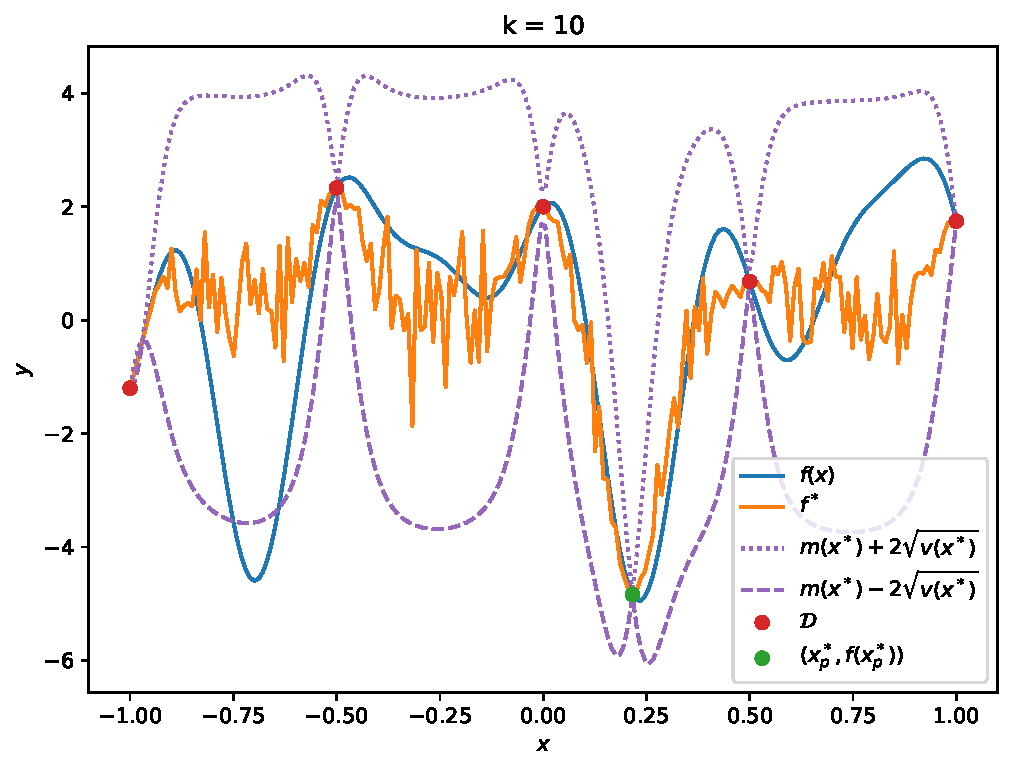
\includegraphics[width=\textwidth]{figures/gp/b2-k_10.pdf}
    \caption{Result of the Bayesian optimization loop with RBF kernel at iteration $k = 10$}
\end{figure}
\subsubsection{Results from using other kernels than RBF}
\begin{figure}[H]
    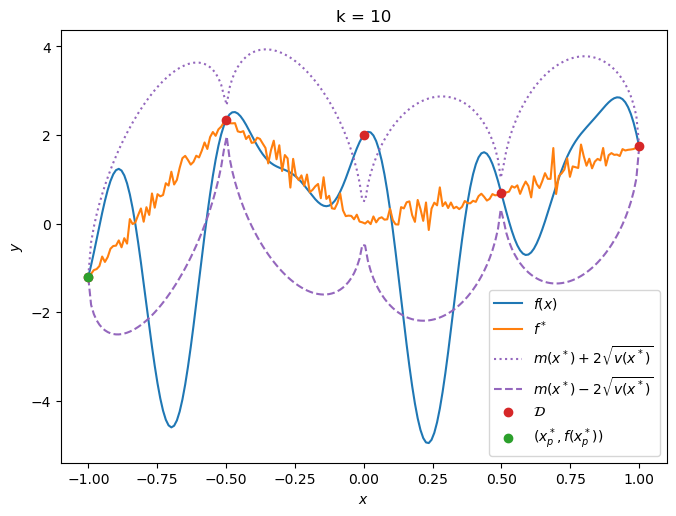
\includegraphics[width=\textwidth]{figures/gp/Brownian.png}
    \caption{Result of running the Bayesian optimization loop with a Brownian kernel}
\end{figure}

\begin{figure}[H]
    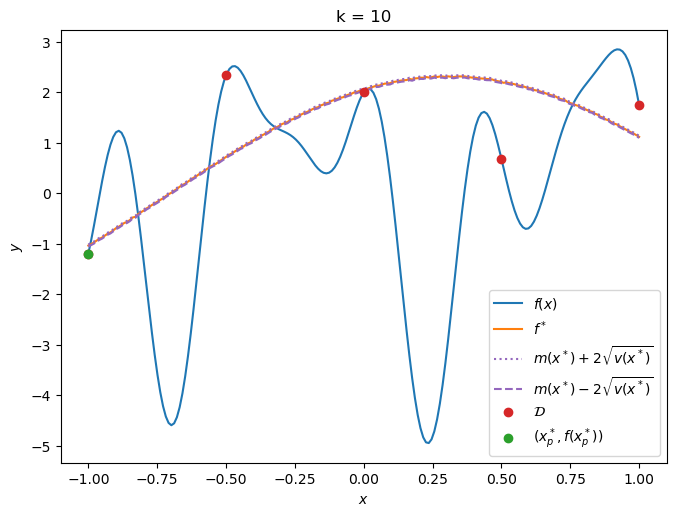
\includegraphics[width=\textwidth]{figures/gp/cosine.png}
    \caption{Result of running the Bayesian optimization loop with a Cosine kernel}
\end{figure}

\begin{figure}[H]
    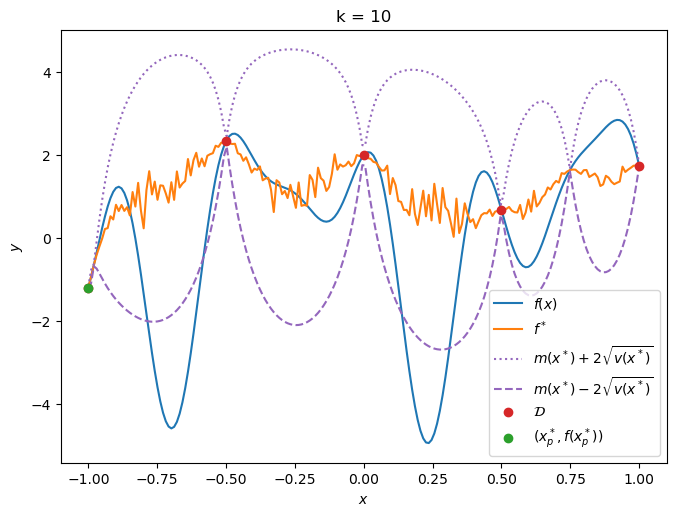
\includegraphics[width=\textwidth]{figures/gp/mattern.png}
    \caption{Result of running the Bayesian optimization loop with a Matern32 kernel}
\end{figure}